\documentclass[12pt]{report}

\usepackage[a4paper,width=150mm,top=25mm,bottom=25mm,bindingoffset=6mm]{geometry}
\usepackage[onehalfspacing]{setspace}
\usepackage{ucs}
\usepackage[table,xcdraw]{xcolor}
\definecolor{mColor1}{rgb}{0.9,0.9,0.9}

\usepackage{fancyhdr}
\pagestyle{fancy}
\fancyhead{}
\renewcommand{\chaptermark}[1]{\markboth{#1}{}}
\renewcommand\sectionmark[1]{\markright{\thesection\ #1}}

\fancyhead[LO, RE]{\leftmark}
\fancyhead[LE, RO]{\rightmark}

\usepackage{titlesec, blindtext, color}
\definecolor{gray75}{gray}{0.75}
\usepackage{mathptmx}
\usepackage[utf8]{inputenc}
\usepackage[T1]{fontenc}
\usepackage[ngerman]{babel}

\usepackage{amsmath,amssymb,amstext,amsthm,mathtools}
\usepackage{url}
\usepackage{caption}
%\usepackage[belowskip=-5pt,aboveskip=0pt]{caption}
\usepackage{subcaption}

\usepackage{float}
\usepackage{lscape}
\usepackage{pdfpages}
\usepackage{rotating}
\usepackage{graphicx}
\setlength\parindent{0pt}
\usepackage{hyperref}
\usepackage{acronym}
\usepackage{textcmds}
\usepackage{longtable}
\usepackage[export]{adjustbox}
\usepackage{upgreek}
\usepackage{dsfont}


\DeclareMathAlphabet{\mathcal}{OMS}{cmsy}{m}{n}
\SetMathAlphabet{\mathcal}{bold}{OMS}{cmsy}{b}{n}

\usepackage{listings, lstautogobble}
\usepackage{textcomp}
\definecolor{yo}{rgb}{0.9,0.6,0}
\definecolor{Gray}{gray}{0.9}
\definecolor{listinggray}{gray}{0.9}
\definecolor{lbcolor}{rgb}{0.95,0.95,0.95}
\lstset{
	backgroundcolor=\color{lbcolor},
	tabsize=4,
	rulecolor=,
	language=python,
        basicstyle=\scriptsize,
        upquote=true,
        aboveskip={1.5\baselineskip},
        columns=fixed,
        showstringspaces=false,
        extendedchars=true,
        breaklines=true,
        prebreak = \raisebox{0ex}[0ex][0ex]{\ensuremath{\hookleftarrow}},
        frame=lines,
        showtabs=false,
        showspaces=false,
        showstringspaces=false,
        identifierstyle=\ttfamily,
        keywordstyle=\color[rgb]{0.55,0,0},
        alsoletter={/,*,[,]},%
        otherkeywords={},
        morekeywords=[2]{with, as},
        morekeywords=[3]{},
        emph={self},          % Custom highlighting
		emphstyle=\color[rgb]{0.1,0.3,1},
		emph={[2]f},          % Custom highlighting
		emphstyle={[2]\color[rgb]{0.1,0.5,0.1}},
		emph={[3]__init__},          % Custom highlighting
		emphstyle={[3]\color[rgb]{0.1,0.3,1}},
		emph={[4]open,str,print,KeyError},          % Custom highlighting
		emphstyle={[4]\color[rgb]{0.2,0.6,0.8}},
        commentstyle=\color[rgb]{0.3,0.3,0.3},
        stringstyle=\color[rgb]{0.133,0.545,0.133},
        	autogobble=true
}
\lstnewenvironment{ttlisting}{\lstset{basicstyle=\scriptsize}}{}

\usepackage{color}
\usepackage[section]{placeins}

\newenvironment{simplechar}{%
	\catcode`\$=12
	\catcode`\&=12
	\catcode`\#=12
	\catcode`\^=12
	\catcode`\_=12
	\catcode`\~=12
	\catcode`\%=12
	\catcode`\"=12
	\catcode`\'=12
	}{}{}

\newtheoremstyle{dotless}{}{}{\itshape}{}{\bfseries}{}{ }{}

\theoremstyle{dotless}

\newtheorem{thm}{Theorem}
\newtheorem{defn}[thm]{Definition} 
\newtheorem{exmp}[thm]{Example}
\theoremstyle{definition}


\begin{document}

\begin{titlepage}
	Warum bin ich nicht einfach Staubsaugervertreter geworden? 
\end{titlepage}

\tableofcontents

\chapter{Allgemeiner Unsinn für Grundlagen aktuarieller Kalkulation}

\subsubsection{Sparten}
\begin{itemize}
	\item Umfasst Leben, Kranken, Komposit, Pensionen
	\item Leben, Kranken, Pensionen sind zusammen Personenversicherung
	\item Komposit: Schaden/Unfall
	\item Besonders: priv. Unfall ist Komposit
\end{itemize}

\begin{defn} (Farny)
	Deckung eines im Einzelnen ungewissen, insgesamt schätzbaren Mittelbedarfs unter Nutzung von Ausgleichsmechanismen im Kollektiv.
\end{defn}

\subsubsection{Wichtigste Zweige Komposit}
\begin{itemize}
	\item Sachversicherung
	\item Haftpflichtversicherung
	\item Transportversicherung
	\item Technische Versicherung
\end{itemize}

\subsubsection{Prämienzahlweise}
\begin{itemize}
	\item üblicherweise jährlich
	\item bei unterjährigen Zahlung Ableitung aus Jahresprämie
\end{itemize}

\subsubsection{Diskont und Barwert}
\begin{itemize}
	\item Diskontfunktion bei einjährigem Zinssatz $r$: $D(t)=(1+r)^{-t}$
	\item Diskontfunktion bei Rechnungszins $i$: $D(t) = (\frac{1}{1+i})^t \eqqcolon v^t$
	\item Barwert aller Leistungen: $L=\sum_{t=0}^{\bar{n}}D(t)\cdot L_t$
	\item Barwert aller Prämien: $P=\sum_{t=0}^{\bar{n}}D(t)\cdot P_t$
	\item Barwert aller Kosten: $K=\sum_{t=0}^{\bar{n}}D(t)\cdot K_t$
\end{itemize}

\subsubsection{Äquivalenzprinzip}
\begin{align}
	\text{(ÄP I):} \ \ \ \ \ \ \ \ \ \ \ \ \ \ \ E(P)=E(L) \\
	\text{(ÄP II):} \ \ E(P)=E(L)+E(K)
\end{align} 

\begin{defn} \ \\
	\begin{itemize}
		\item Falls $L$ und $P$ das Äquivalenzprinzip erfüllen, dann hei{\ss}t $P_{\bullet}$ Nettorisikoprämienprozess und $P_t$ Nettorisikoprämie.
		\item $L$ und $P$ erfüllen ÄP und $\exists \ w_t$ Wahrscheinlichkeit der Prämienzahlung $P_t$ und $\bar{P}$ konstant mit $E(P_t)=\bar{P}\cdot w_t \ \forall \ t \in \{0,...,\bar{n}\}$. $\bar{P}$ konstante Nettorisikoprämie.
		\item Bruttorisikoprämie: $P^+ \coloneqq \bar{P}+c$ mit $c>0$ Sicherheitszuschlag.
		\item Alternativ: Sicherheitszuschlag bereits in Nettorisikoprämie enthalten
	\end{itemize}
\end{defn}

\subsubsection{Notation}
\begin{itemize}
	\item $\bar{n}$: Modelldauer
	\item $t$: Zeit in jahren
	\item $r$: einjähriger konstanter Zinssatz
	\item $D(t)$: Diskontfunktion
	\item $L_t$: Versicherungsleistung in $t$
	\item $q_t$: Eintrittswahrscheinlichkeit Leistungsfall in $t$
	\item $P_t$: Prämienzahlung in t
	\item $w_t$: Wahrscheinlichkeit Prämienzahöung in $t$
	\item $K_t$: Kosten in $t$
	\item $L$: Leistungsbarwert
	\item $P$: Prämienbarwert
	\item $K$: Kostenbarwert
\end{itemize}

\subsubsection{Sterbetabeln}

\begin{figure}[ht]
	\centering
	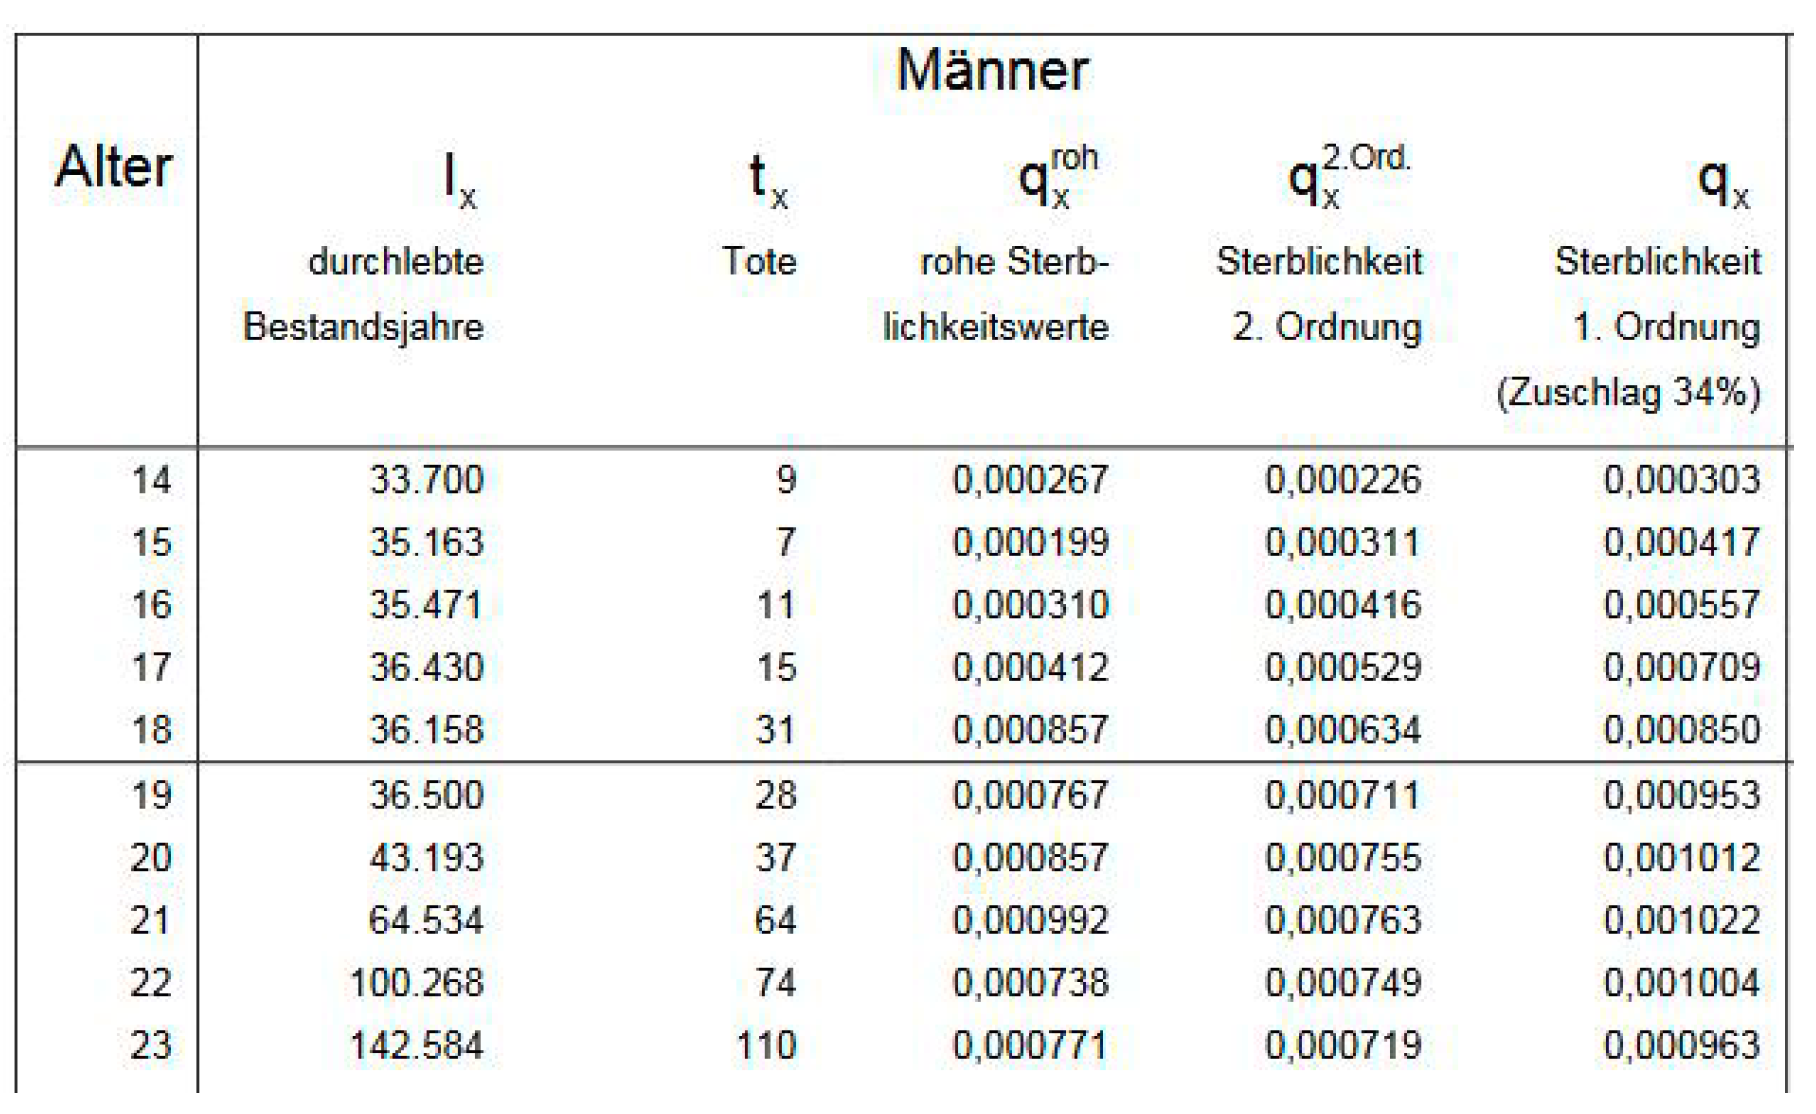
\includegraphics[width = .8\textwidth]{Bilder/Sterbetafelbsp.png}
\end{figure}

\subsubsection{Allgemeine aktuarielle Herangehensweise, spartenübergreifend ähnliches Standardvorgehen zur Bewertung zufälliger zukünftiger Versicherungsleistungen}
\begin{itemize}
	\item Beobachtung von Vergangenheit (Daten) zur Vorhersage der Zukunft
	\item Anpassung geeigneter Wahrscheinlichkeitsverteilung
	\item Sorgfalt bzgl. möglicher Änderungen von Annahmen im zeitlichen Verlauf
	\item typischerweise konstante Prämienhöhe
	\item Risiko steigt mit zeitlichem Verlauf
	\item Ansparprozess und Entsparprozess
\end{itemize}

\subsubsection{Rückstellungen}
\begin{itemize}
	\item Ziel: Sicherstellung der dauernden Erfüllbarkeit
	\item versicherungstechnische Rückstellungen wichtigste Passivposition in der Bilanz des VU
	\item hohe bedeutung für interne Unternehmensbewertung
	\item Einfluss auf Besteuerung des VU
	\item Unterschied zwischen bilanzieller und einzelvertraglicher versicherungsmathematischer Deckungsrückstellung
	\item Deckungskapitel $\hat{=}$ Erwarteter Barwert künftiger Leistungen - Erwarteter Barwert künftiger Beiträge
\end{itemize}

\subsubsection{Rückstellungen in der Schadenversicherung}
\begin{itemize}
	\item Einzelschadenreserven: für noch nicht vollständig abgewickelte Schäden
	\item Deckungsrückstellungen: für Haftpflicht, Unfallrenten und Beitragsrückgewähr in Unfall
	\item Spätschadenpauschalreserve: für IBNR
	\item Schwankungsrückstellung: relevant für Zweige mit stark variierenden Schadenfällen 
\end{itemize}

\subsubsection{Prämienprinzipien}
\begin{itemize}
	\item Ziel: Zuordnung angemessener Prämie durch Bemessung geeigneter Sicherheitszuschläge
	\item Deckung der Leistungsfälle und zusätzliche Prämie zur Bereitschaft der Risikoübernahme durch VU (Sicherheitszuschlag SZ(X))
	\item Prämienprinzipien $H(X) \coloneqq E(X)+SZ(X)=P^+$, $X$ ist das versicherte Risiko
	\item Sicherheitszuschlag bei gleichem EW höher, wenn Risiko gefährlicher
	\item Nettorisikoprinzip: $H(X)=E(X)$
	\item Erwartungswertprinzip: $H(X)=E(X)+\delta \cdot E(X) = (1+\delta) \cdot E(X)$
	\item Varianzprinzip: $H(X)=E(X) + \delta \cdot Var(X)$
	\item Standardabweichungsprinzip: $H(X)=E(X) + \delta \cdot \sqrt{Var(X)} = E(X) + \delta \cdot \sigma(X)$
	\item Exponentialprinzip: $H(X) = \frac{1}{a} \cdot ln(M_X(a)) = \frac{1}{a}\cdot ln(E[e^{aX}])$ mit $a>0$, Monumenterzeugender Funktion $M_X$, entspricht näherungsweise Varianzprinzip mit $\delta = \frac{a}{2}$
\end{itemize}

\begin{defn}
	(Ungleichung von Centelli)
	$P(X>E(X)+c) \leq \frac{Var(X)}{c^2+Var(X)}$ \\
	Hinweis: SZ wird hier stark überschätzt.
\end{defn}

\subsubsection{Beispiele Risikoma{\ss}e}
\begin{itemize}
	\item Erwartungswert $E(X)$
	\item Varianz $Var(X)$
	\item Schiefe $\gamma(X)$ (Symmetriema{\ss}
	\item Tail-Whk $P(X>t)$
	\item Ruin- und Verlustwahrscheinlichkeiten
	\item Bernoulli-Nutzen
	\item Value at Risk (VaR), Expected Shortfall, Tail Value at Risk (TVaR)
\end{itemize}

\begin{defn}
\begin{align}
	\text{Additivität: } H(X+Y)=H(X)+H(Y) \ \forall \ X,Y \text{stochastisch unabhängig} \\
	\text{Subadditivität: } H(X+Y) \leq H(X)+H(Y) \ \forall \ X,Y \text{stochastisch unabhängig} \\
	\text{Erwartungswertübersteigend: } SZ(X) \geq 0
\end{align}
\end{defn}

% To-Do: Folie 112-114 beantworten und einfügen

\begin{defn}
	(1) Ein Kollektiv stellt eine Zusammenfassung von Risiken dar, die durch gleichartige Gefahren bedrohnt sind. Kollektiv bedeutet nicht zwangsläufig, dass es sich um \textit{versicherte Risiken} handelt. \\
	(2) Der Risikoausgleich im Kollektiv stellt neben dem Ausgleich in der Zeit ein wesentliches Funktionsprinzip von Versicherungen dar. \\
	(3) Ein Kollektiv hei{\ss}t homogen, falls alle Risiken des Kollektivs dieselbe Verteilung besitzen, anderenfalls hei{\ss}t es heterogen. \\
	(!) Hinweis: Homogenität und Unabhängigkeit sind keine notwendige Voraussetzung für Risikoausgleich im Kollektiv. Im Gegenteil: gleicht sich durch gegenläufige Abhängigkeiten z.T. aus.
\end{defn}

\subsubsection{Risikoausgleich}
\begin{itemize}
	\item Das Überschreiten einer prozentualen Maximalabweichung vom Erwartungswert wird bei wachsendem Kollektiv immer unwahrscheinlicher.
	\item Risikoausgleich im Kollektiv erfolgt insofern, als dass der Variationskoeffizient als versicherungsspezifisches Risikoma{\ss} für wachsende Bestände gegen 0 konvergiert.
	\item Mit zunehmender Zahl von Risiken sinkt die relative Abweichung des arithmetischen Mittels vom Erwartungswert.
\end{itemize}

\begin{defn}
$Y_i\geq$ kumulierter Gesamtaufwand des $i$-ten Risikos. $S^{ind}=\sum_{i=1}^nY_i $.
	\begin{align}
		\text{Durch Linearität des EWs: } E(S^{ind})=\sum_{i=1}^n E(Y_i) \\
		\text{Da } Y_i \text{ unabhängig: } Var(S^{ind})=\sum_{i=1}^n Var(Y_i) \\
		\text{Variationskoeffizient: } Vko(S^{ind})=\frac{\sqrt{\sum_{i=1}^nVar(Y_i)}}{\sum_{i=1}^nE(Y_i)}
	\end{align}
\end{defn}

\begin{defn}
	Erste und zweite Formel von Wald. N die Schadenzahl. \\
	(1) $E(S^{koll})=E(N)\cdot E(X)$ \\
	(2) $Var(S^{koll})=E(N) \cdot Var(X) + (E(X))^2 \cdot Var(N)$
\end{defn}

\subsubsection{Gegenüberstellung individuelles und kollektives Modell}
\begin{itemize}
	\item dieselbe Gesamtsumme $S^{int}=S^{koll}$
	\item im individuellen Modell Aggregation der einzelnen Aufwände pro Risiko und Zeitraum erforderlich
	\item kollektives Modell: Betrachtung einzelner Ereignisse ohne Erfassung, welches Risiko den Aufwand verursacht
	\item i.A. bietet das KM eine bessere Basis für die Schätzung der Verteilung
	\item Annahme identisch verteilter Aufwände bei IM nur näherungsweise erfüllt 
\end{itemize}


\subsubsection{Zustandsmodell der Personenversicherung}

\begin{figure}[ht]
	\centering
	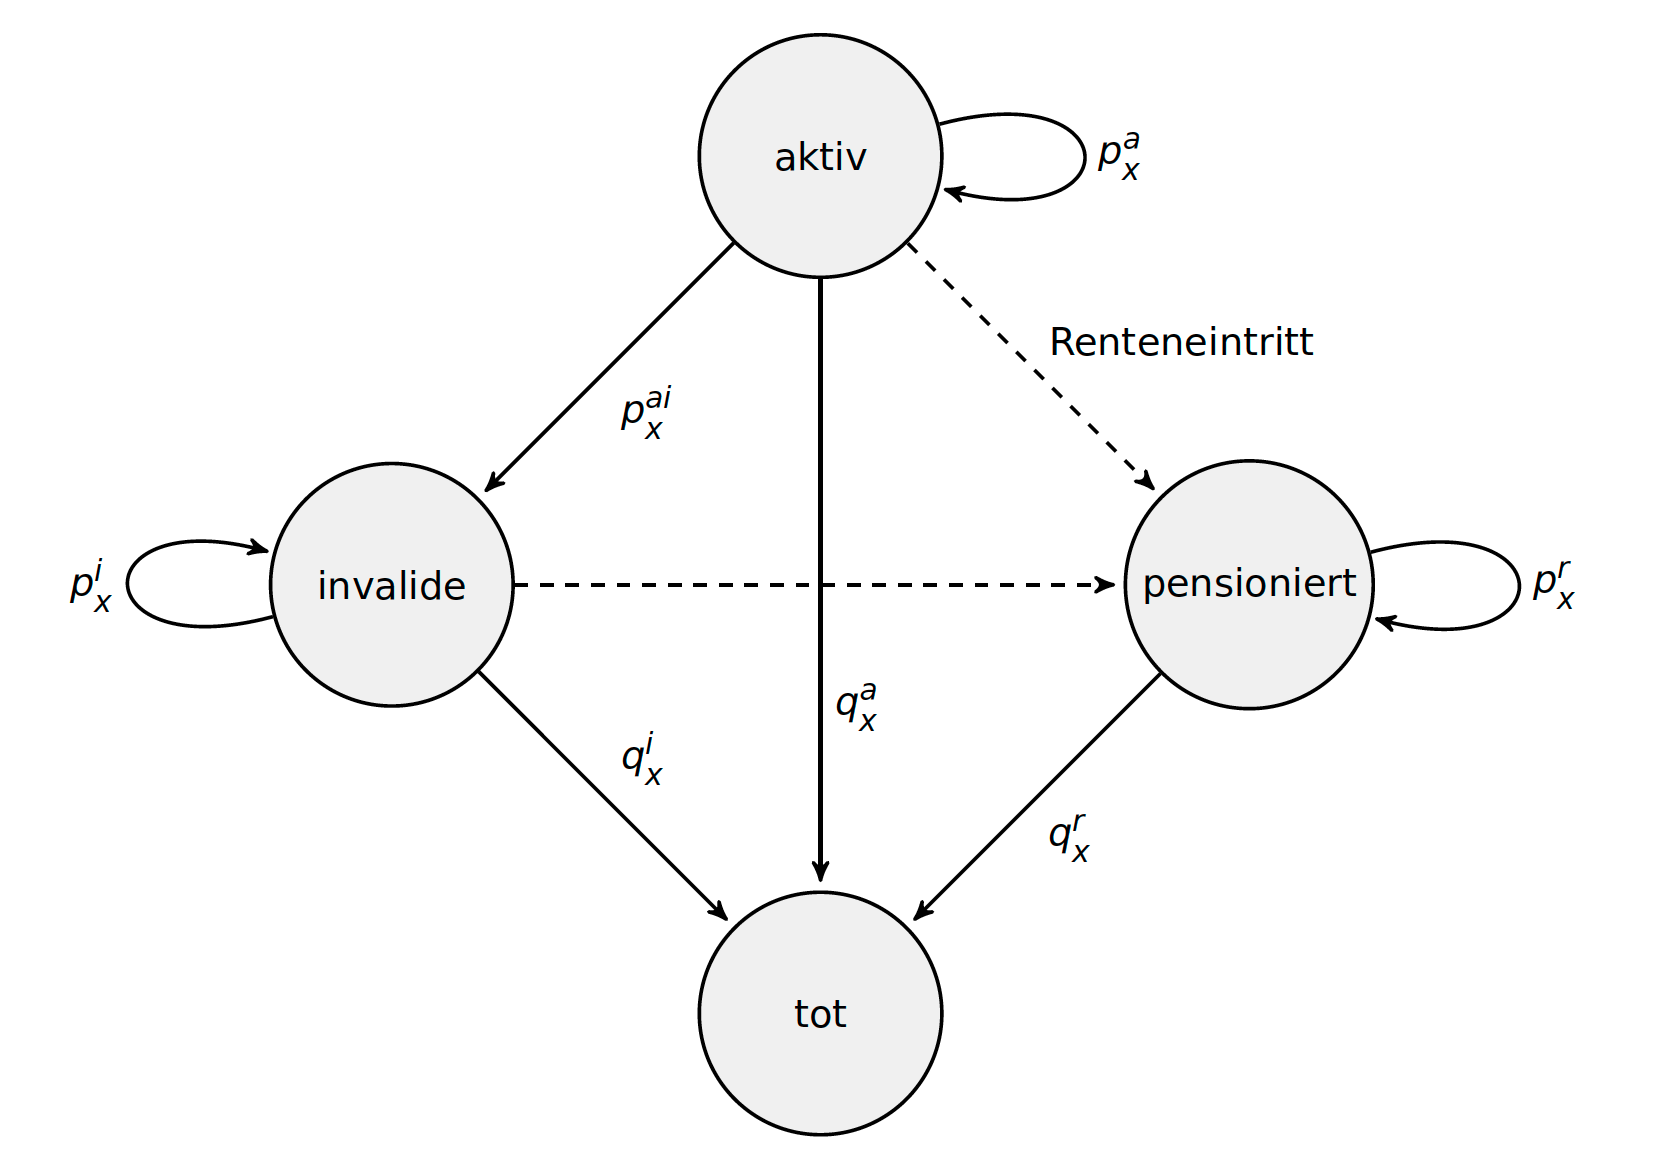
\includegraphics[width = .8\textwidth]{Bilder/ZustandsmodellPersVers}
\end{figure}
 \begin{itemize}
 	\item Modellannahmen nicht immer sachgerecht
 	\item Markov-Eigenschaft kritisch: Relevant, ob \textit{aktiv} $\rightarrow$ \textit{Rente} oder \textit{invalide} $\rightarrow$ \textit{Rente}
 	\item z.T. sehr viele Zustände erforderlich (z.B. Abhängigkeit der Leistungshöhe von Anzahl Dienstjahren, bei Invalidität der Zeitpunkt des Eintritts in den Invalidenstatus)
 \end{itemize}

\subsubsection{Risikoteilung}

\begin{itemize}
	\item teilweiser Risikotransfer im direkten Geschäft zwischen VN und Erstversicherer sowie im Rahmen von Rückversicherung (RV)
	\item Risikoteilung im Direktgeschäft: Selbstbehalt beim VN, genannt \textit{Franchisen}
	\item in der Rückversicherung: Selbstbehalt beim Erstversicherer, genannt \textit{Prioritäten}
	\item risikopolitisch und nicht gewinnorientierte Vorgehensweise
	\item für den Erstversicherer:
		\begin{itemize}
			\item Verringerung des versicherungstechnischen Risikos
			\item Erhöhung Zeichnungskapazität
			\item Solvenzverbesserung
			\item Kapitalkostenreduktion
		\end{itemize}
	\item für den Rückversicherer:
		\begin{itemize}
			\item Existenzgrundlage
			\item bessere Diversifikation der Risiken als beim Erstversicherer
		\end{itemize}
\end{itemize}

\subsubsection{Begrifflichkeiten Rückversicherung}
\begin{itemize}
	\item aktive RV: Angebot von Rückversicherungskaapzitäten
	\item passive RV: Nachfrage nach RV-Schutz durch Erstversicherer
	\item Retrozession: Weitergabe in Rückdeckung genommener Risiken eines RV an anderen RV
	\item obligatorische RV: Verpflichtung des Erstversicherers zur Übertragung aller vertraglich definierten Risiken ohne Ablehnungsrecht des RV
	\item fakultative RV: individuelle Abgabe und Annahme von Risiken auf einzelvertraglicher Basis
	\item Originalbasis: RV erhält anteilig Prämie und muss Deckungskapital bilden
	\item Risikobasis: RV erhält Risikobeitrag und bildet kein Deckungskapital
\end{itemize}

\subsubsection{Proportionale Risikoteilung}
\begin{itemize}
	\item proportionale Aufteilung der Schäden in festem Verhältnis zwischen Vertragspartnern
	\item Proportionen vorab fest und unabhängig von Schadenhöhen
	\item einfache Struktur, geringe Flexibilität
	\item bei RV Schicksalsteilung: Übernahme von Teilen des Erstversicherungsrisikos, aber nicht kaufmännischen oder unternehmerischen Risikos des Erstversicherers
	\item wichtigste Formen der proportionalen RV: Quotenrückversicherung, Summenexedentenrückversicherung
		\begin{itemize}
			\item QRV: feste Quotenabgabe $q$, Selbstbehalt $ \underbar{$S^{ind}$} = (1-q) \cdot S^{ind}$
			\item SERV: Festlegung eines Maximums $v_0$ als maximaler Selbstbehalt des Erstversicherers bei jedem einzelnen Risiko und vertragsindividuelle Quote $q_i = \frac{max\{v_i-v_0, \ 0\}}{v_i}$ in Abhängigkeit der jeweiligen Versicherungssumme
		\end{itemize}
	\item SERV dient der Homogenisierung des Portfolios und der Reduktion von Spitzenrisiken
	\item Üblicherweise Haftungsbegrenzung für RV i.H.v. Vielfachem $m$ von $v_0$. Mehrere aneinandergereiht, s.d. man Layering erhält.
\end{itemize}






\chapter{Schadenversicheungsmathematik}

\subsubsection{Notation}
\begin{itemize}
\item $n$: Anzahl der Verträge
\item $\alpha_i$: Jahreseinheit des $i$-ten Vertrages, $i=1,...,n$
\item $v_i$: Versicherungssumme des $i$-ten Vertages
\item $b_i$: Jahresbeitrag des $i$-ten Vertrages
\item $N$: (zufällige )Anzahl Schäden
\item $X_j$: (zufällige) Höhe des $j$-ten Einzelschadens, $j=1,...,N$
\end{itemize}

\subsubsection{Schadenkennzahlen}
\begin{itemize}
\item Schadendaten: Zeitpunkt, Art und Ursache, Sachlicher Bezug, Ort, Entschädigung
\item Bestandsdaten: Versicherungssumme, persönliche Daten der VN, ...
\item Exposure: Das Risiko eines Vertrags oder eines Bestandes\\
Exposuremaß: versicherungstechnische Risiko bzw Schadenbedarf eines Bestandes (Bsp: Jahreseinheiten, Anzahl Risiken, Summe Beiträge, ...)
\item Anzahl Jahreseinheiten bzw. durchschnittliche Anzahl der Verträge: $n_0 := \sum_{i=1}^{n} \alpha_i$
\item Schadenhäufigkeit / Frequenz: $H:= \frac{\text{Anzahl Schäden}}{\text{Anzahl Jahreseinheiten}} = \frac{N}{n_0}$
\item Schadendurchschnitt: $D:= \frac{\text{Gesamtschaden}}{\text{Anzahl Schäden}} := \frac{\sum_{j=1}^N X_j}{N} = \frac{S}{N}$
\item Schadenbedarf: $SB:= \frac{\text{Gesamtschaden}}{\text{Anzahl Jahreseinheiten}} = \frac{S}{n_0} = H\cdot D = \text{Schadenhäufigkeit} \cdot \text{Schadendurchschnitt}$
\item Summe verdiente Beiträge: $b:= \sum_{i=1}^n \alpha_i \cdot b_i$
\item Schadenquote: $SQ:=\frac{\text{Gesamtschaden}}{\text{Summe verd. Beiträge}} = \frac{S}{b}$
\item durchschnittliche kumulierte Versicherungssumme: $v:= \sum_{i=1}^n \alpha_i \cdot v_i$
\item Schadensatz: $SS:=\frac{\text{Gesamtschaden}}{\text{durchschn. kumulierte V-Summe}} = \frac{S}{v}$
\item durchschnittliche Versicherungssumme: $v_0:= \frac{\text{durchschn. kumulierte V-Summe}}{\text{Anzahl Jahreseinheiten}} = \frac{v}{n_0}$
\item Schadengrad: $SG:=\frac{\text{Schadendurchschnitt}}{\text{durchschn. V-Summe}} = \frac{D}{v_0}$
\end{itemize}


















\end{document}